\setcounter{mtc}{5} %indique le numéro réel du chapitre, pour la mini table des matières
\chapter{Project Overview}
\minitoc  %insert la minitoc

\graphicspath{{Chapitre1/figures/}}
%==============================================================================
\pagestyle{fancy}
\fancyhf{}
\fancyhead[R]{\bfseries\chaptername~\thechapter. }
\fancyfoot[R]{\thepage}
\renewcommand{\headrulewidth}{0.5pt}
\renewcommand{\footrulewidth}{0pt}
%\renewcommand{\chaptermark}[1]{\markright{\MakeUppercase{\chaptername~\thechapter. #1 }}{}}
%\renewcommand{\sectionmark}[1]{\markright{\thechapter.\thesection~ #1}}

\begin{spacing}{1.2}
%==============================================================================

\section*{Introduction}
This opening chapter establishes the foundation of the graduation project by introducing the
host company and defining the project’s scope. We examine the organizational context,
outline the main objectives and challenges, and present the methodological framework that
guides the development process.


\section{Host Company: Google} 

\subsection{Presentation} 
Founded in 1998, Google LLC is a global leader in technology and innovation~\cite{google2024company}. As a subsidiary of Alphabet Inc., Google's mission is to organize the world's information and make it universally accessible and useful. Guided by values such as innovation, accessibility, sustainability, and user trust, Google establishes itself as one of the most influential companies shaping the digital era. Its culture emphasizes collaboration, diversity, inclusion, and impact-driven engineering, enabling continuous leadership in research and product development.

Figure~\ref{fig:google_logo} shows the Google logo.

\begin{figure}[!ht]\centering

\includegraphics[scale=0.06]{Images/google_logo.png}
\caption{Google Logo}
\label{fig:google_logo}
\end{figure}

\subsection{Products and services} 
Google offers a broad ecosystem of products and services that touch nearly every aspect of digital life. Among its flagship consumer products are Google Search, Maps, Gmail, Chrome, and the Android operating system, serving billions of users daily. 

Beyond consumer services, Google develops enterprise and cloud-based solutions such as Google Cloud Platform and Google Workspace, as well as advanced AI systems like Vertex AI. The company also invests in hardware, including Pixel devices, Nest smart home products, and ChromeOS. 

These products reflect Google's commitment to connecting people, improving productivity, and driving digital transformation worldwide.

Figure~\ref{fig:google_products} provides an overview of some Google products.

\begin{figure}[!ht]\centering
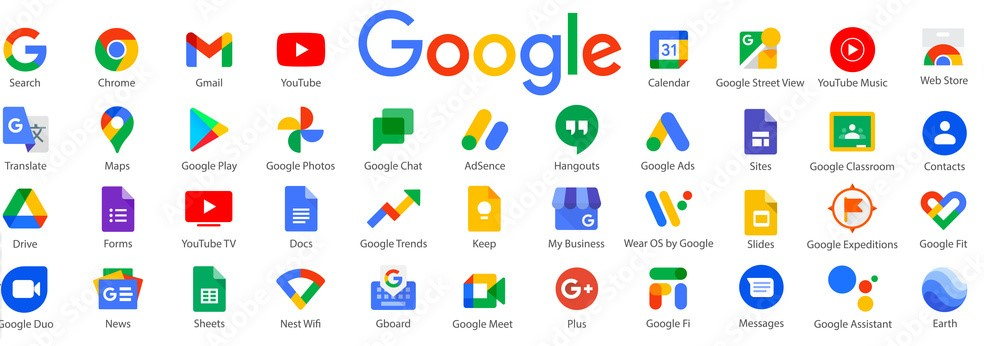
\includegraphics[scale=1.3]{Images/google_products.jpg}
\caption{Overview of some Google products}
\label{fig:google_products}
\end{figure}

\subsection{Focus Area} 
\subsubsection{YouTube}
Acquired by Google in 2006~\cite{youtube2024platform}, YouTube becomes the world's leading video-sharing platform, serving more than two billion logged-in users monthly. It empowers individuals to create, share, and discover video content globally while sustaining a vibrant creator economy. From a technical perspective, YouTube integrates video processing, recommendation systems, live streaming, advertising, and trust and safety to deliver a seamless experience across devices.

Figure~\ref{fig:youtube_logo} displays the YouTube logo.

\begin{figure}[!ht]\centering

\includegraphics[scale=0.06]{Images/youtube_logo.png}
\caption{YouTube Logo}
\label{fig:youtube_logo}
\end{figure}

\subsubsection{YouTube Developer Infrastructure Team}
Within YouTube’s engineering organization, the Developer Infrastructure (Dev Infra) team supports thousands of engineers building the platform. The team develops tooling, automation, and guidelines that improve efficiency, reliability, and consistency in software development. By maintaining developer velocity and quality at scale, the Dev Infra team contributes directly to YouTube’s ability to innovate and grow.




\section{Project Overview}

\subsection{Project Context}
This project develops within the scope of a development infrastructure team dedicated to supporting developers by providing tools and extensions that enhance their daily workflows. As part of this mission, the team explores how artificial intelligence can be leveraged to assist developers in maintaining code quality and adhering to best practices. The goal is to investigate how large language models (LLMs) can complement traditional approaches by offering more intelligent and context-aware guidance directly within the IDE.  

In parallel, this work also constitutes the mandatory end-of-studies-internship project required for obtaining the software engineering degree at the National Institute of Applied Science and Technology, providing both academic and practical significance.  

\subsection{Problem Statement}
In large-scale software development environments, maintaining uniform adherence to \textbf{internal framework–specific guidelines} across multiple teams is crucial for ensuring code quality, consistency, and long-term maintainability. While modern development environments provide assistance for general programming practices or widely used frameworks, they lack intelligent support for the nuanced, evolving rules of internal frameworks. As a result, developers often receive feedback on internal best practices only during code reviews, after significant effort has already been invested. This delayed feedback cycle leads to inefficiencies such as rework, slower iterations, and frustration among teams who must refactor code that was previously considered complete. The absence of real-time, context-aware guidance tailored to internal frameworks leaves developers navigating complex design decisions without adequate support, leading to technical debt, inconsistent quality, and higher onboarding complexity. Addressing this gap requires solutions that proactively enforce internal framework best practices during the coding phase, providing timely and context-specific feedback directly within the IDE.  

\subsection{Proposed Solution}
This project introduces an \textbf{AI-assisted feedback system integrated directly into the coding workflow}. The solution is designed to address the challenges outlined above through three key capabilities:  

\begin{itemize}
    \item \textbf{Shift-Left Feedback:} Provide developers with earlier, context-aware guidance during the coding phase, ensuring that issues are detected and addressed well before code reviews.  
    \item \textbf{Framework-Specific Best Practice Enforcement:} Surface adherence to internal framework guidelines early in the development process, going beyond syntax and correctness.  
    \item \textbf{Reduced Review Burden:} Shift part of the best practice enforcement from manual reviews to the authoring stage, allowing reviews to focus on higher-level insights.  
\end{itemize}

By integrating intelligent, framework-aware feedback directly into the coding workflow, this solution aims to minimize rework, improve adherence to internal standards, and accelerate development velocity.  

\section{Work Methodology}

\subsection{Agile Development Approach}
Agile software development, as defined by Beck et al.~\cite{beck2001agile}, emphasizes "individuals and interactions over processes and tools, working software over comprehensive documentation, customer collaboration over contract negotiation, and responding to change over following a plan." This methodology is adopted to support iterative development and maintain flexibility in responding to evolving requirements. According to Martin~\cite{martin2003agile}, agile practices enable continuous integration of feedback, ensuring that each increment of work aligns with both technical goals and the broader product vision. Testing, validation, and code reviews are incorporated throughout the process to maintain high quality, while frequent collaboration provides clarity and shared ownership of outcomes. Agile principles complement the focus on engineering excellence, including rigorous design reviews, thorough testing, robust code reviews, and DevOps-enabled automation.

\subsection{Kanban Workflow}
Kanban, as described by Anderson~\cite{anderson2010kanban}, is "a method for managing knowledge work with an emphasis on just-in-time delivery while not overloading the team members." The dynamic workload of the development infrastructure team, including feature requests, bug fixes, and maintenance tasks, is managed using this Kanban workflow. According to Kniberg and Skarin~\cite{kniberg2011kanban}, Kanban enables teams to visualize tasks and limit work in progress, preventing bottlenecks and allowing quick focus shifts to urgent issues when necessary. Work is structured into stages to maintain clear coordination while allowing the flexibility to adapt priorities as requirements evolve.  

The Kanban workflow includes the following stages, as illustrated in Figure~\ref{fig:kanban_workflow}:

\begin{itemize}
    \item \textbf{Backlog:} Prioritized collection of feature requests, enhancements, and bug fixes.
    \item \textbf{Research \& Design:} Assessment of technical feasibility and preparation of design specifications.
    \item \textbf{Development:} Implementation and integration of features into the system.
    \item \textbf{Review \& Testing:} Code review, unit tests, and integration tests to ensure quality and correctness.
    \item \textbf{Deployment:} Release of validated features to developer environments.
\end{itemize}

\begin{figure}[H]
    \centering
    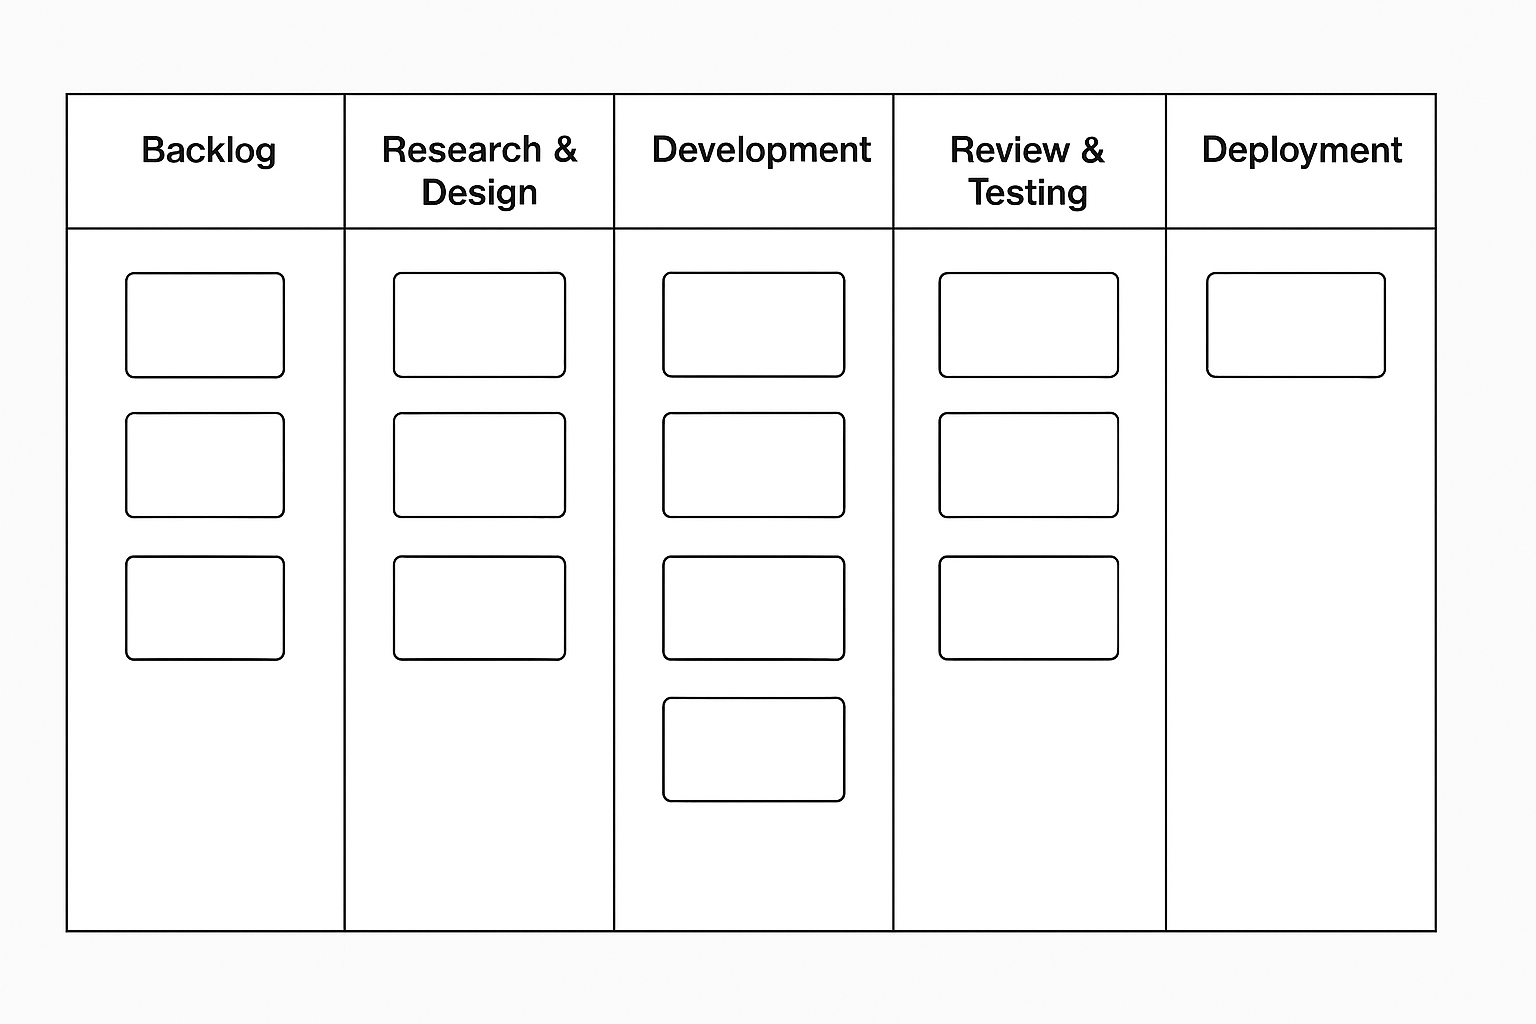
\includegraphics[scale=0.2]{Images/kanban.png}
    \caption{Kanban Workflow}
    \label{fig:kanban_workflow}
\end{figure}


\subsection{Development Process}
The project follows an iterative engineering cycle designed to balance thorough planning with incremental delivery, as illustrated in Figure~\ref{fig:development_cycle}. This cycle guides the work through structured stages, supported by dedicated tools and regular collaboration:

\begin{figure}[H]
    \centering
    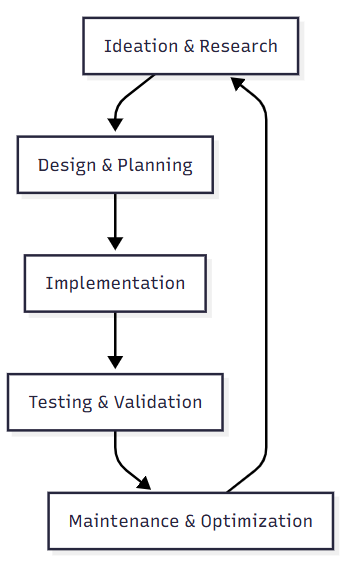
\includegraphics[scale=0.5]{Images/dev_process.png}
    \caption{Project Development Cycle}
    \label{fig:development_cycle}
\end{figure}

The main stages, as depicted in the figure, include:

\begin{itemize}
    \item \textbf{Onboarding and Initial Tasks:} The project begins with a structured onboarding phase, where familiarization with internal tools, repositories, and coding standards combines with the resolution of assigned bugs. This phase ensures a smooth transition into the team's workflow and provides early practical experience.

    \item \textbf{Ideation and Research:} Following onboarding, the project enters an exploration phase to clarify objectives, gather requirements, and investigate potential solution directions. Independent research complements collaborative discussions to assess feasibility and align priorities.

    \item \textbf{Design and Planning:} A detailed design document is authored to present technical choices, architectural considerations, and the proposed workflow. The document undergoes iterative review by engineers, and the final approved plan is transferred to the internal task management system for structured tracking and prioritization.

    \item \textbf{Implementation:} Development is performed in small, reviewable increments using the internal development environment within the company-wide repository. Each change is submitted with unit tests and validated through manual and AI-assisted code reviews.

    \item \textbf{Testing and Validation:} Functionality and reliability are verified continuously. Automated unit tests ensure correctness at the component level, while integration reviews and structured evaluations validate the behavior within the larger system.

    \item \textbf{Maintenance and Optimization:} Refactoring, bug fixes, and updates are performed throughout development, particularly as dependencies evolve or methods become deprecated. This ensures that the solution remains consistent, maintainable, and aligned with evolving standards.
\end{itemize}

Collaboration is supported through a structured communication rhythm, combining regular syncs with the host and co-host, weekly team meetings, and occasional cross-team discussions. This cadence provides timely feedback, clear guidance, and alignment on shared dependencies throughout the iterative cycle.


\subsection{Project Timeline}
The project spans four months (May 5 – September 5, 2025). Work is scheduled based on business priorities and technical dependencies. Early weeks focus on research and design, followed by implementation, testing, and iterative refinement.

Figure~\ref{fig:project_timeline} shows the detailed project timeline.

% Landscape page for timeline
\newpage
\begin{landscape}
    \vspace*{\fill}
    \begin{figure}[!ht]
        \centering
        \begin{ganttchart}[
            hgrid,
            vgrid,
            time slot format=isodate,
            x unit=0.13cm,           % slightly smaller for horizontal fit
            bar height=1.10,
            y unit chart=1.20cm,
            y unit title=1.40cm,
            title height=1.2,
            title/.append style={font=\Large},
            bar label font=\small,
            group label font=\small,
            milestone label font=\small,
            group/.append style={fill=black!20},
            bar top shift=0.8,       % push bars down
        ]{2025-05-05}{2025-09-05}

            \gantttitlecalendar{month=name} \\  % month names

            \ganttgroup{Onboarding}{2025-05-05}{2025-05-18} \\
            \ganttgroup{Research \& Ideation}{2025-05-19}{2025-06-01} \\
            \ganttgroup{Design \& Planning}{2025-06-02}{2025-06-15} \\
            \ganttgroup{LLM Agent Development}{2025-06-16}{2025-07-15} \\
            \ganttgroup{Core Integration in Extension}{2025-07-16}{2025-07-31} \\
            \ganttgroup{UI \& Workflow Testing}{2025-08-01}{2025-08-21} \\
            \ganttgroup{Documentation}{2025-08-22}{2025-08-28} \\
            \ganttgroup{Presentation \& Feedback}{2025-09-01}{2025-09-04} \\
            \ganttgroup{Tuning \& Maintenance}{2025-06-16}{2025-08-21}

        \end{ganttchart}
        \caption{Project Timeline - Detailed Schedule}
        \label{fig:project_timeline}
    \end{figure}
    \vspace*{\fill}
\end{landscape}



\section*{Conclusion}
In summary, this chapter outlines the project's context by presenting the host company, defining the problem, and clarifying the main objectives and challenges. It also describes the methodology chosen to guide the work, which provides the basis for the technical developments detailed in the following chapters.



%==============================================================================
\end{spacing}
